При детальном анализе временной задержки между изображениями гравитационно линзированных сверхновых нельзя пренебречь \textit{микролинзированием} - линзированием на отдельных звёздах или других компактных объектах в галактике-линзе. Его масштабы, то есть характерные углы отклонения света, в миллион раз меньше масштабов сильного линзирования. На текущий момент разрешить множественные изображения, возникающие в результате микролинзирования не представляется возможным. Однако вполне возможно “засечь” этот эффект благодаря кратковременному увеличению или ослаблению яркости источника. Микролинзирование не вносит существенный вклад в наблюдаемую кривую блеска, если размер источника сильно превышает радиус Эйнштейна $\theta_E$ для звезды-микролинзы. Напомним, что эта величина задаётся соотношением:

\begin{equation}\tag{\ref{eq:r_ein}}
\theta_{E}=\sqrt{\frac{4 G M}{c^{2}} \frac{D_{d s}}{D_{d} D_{s}}}.
\end{equation}

Известно, что для источников с угловым размером $\theta > 5\theta_E$ значение обусловленной микролинзированием добавки к звёздной величине обратно пропорционально $\theta$ (\cite{refsdalstabell1991}). Для конфигурации SN Refsdal оценим $\theta_E$ для звезды с массой $1 M_{\odot}$. Расстояния до галактики-линзы (члена скопления MACSJ1149.6+2223, $z_d=0.54$), до источника ($z_Ss=1.49$), а также между линзой и источником равны, согласно формуле \eqref{eq:ang_dia_dist}, 
$$ D_d=D_A(0,z_d)=1311.54 \ \textrm{МПк}, $$
$$ D_s=D_A(0,z_s)=1744.81 \ \textrm{МПк}, $$
$$ D_{ds}=D_A(z_d,z_s)=932.47 \ \textrm{МПк}, $$
соответственно. В результате, радиус Эйнштейна для звезды с массой $1 M_{\odot}$ составляет, согласно формуле \eqref{eq:r_ein}, $$\theta_E \approx 1.8 \cdot 10^{-6} \ ''. $$ 

Для сверхновых II типа максимальный размер фотосферы составляет $R_{SN} \sim 10^{15}$ см (\cite{razmer}). По результатам гидродинамического моделирования расширения оболочки SN Refsdal её максимальный размер составляет $R_{SN} = 1.75\cdot10^{15}$ см (\cite{petrnat2020}), или, в угловых единицах, $$\theta_{SN} = \frac{R_{SN}}{D_S} \approx 6.7 \cdot 10^{-8} \ '' =  0.037 \cdot \theta_E $$  Таким образом, угловой размер SN Refsdal не превышает характерный радиус Эйнштейна, а значит, микролинзирование может вносить существенные искажения в её кривые блеска. %Эта оценка пригодится нам немного позже для оценки масштаба карт.

В данной работе для изучения микролинзирования используется вычислительная программа {\tt{microlens}} (\cite{wambsganss1990-thesis}, \cite{wambsganss1999}), которая моделирует методом обратной трассировки лучей (\textit{inverse ray shooting}, \cite{kayserrefsdal1986}) распределение каустик в плоскости источника, основываясь на распределении звёзд в плоскости линзы. Выходными данными этой программы являются карты микрокаустик - двумерные массивы, каждый пиксель которых содержит значения обусловленного микролинзированием усиления в плоскости источника. Основными входными параметрами для каждой карты являются безразмерные поверхностные плотности звёзд $\kappa_*$ и непрерывно распределенной тёмной материи $\kappa_c$ в линзирующей галактике\footnote{Либо параметр $s=\kappa_c/(\kappa_*+\kappa_c)$.}, внешний сдвиг $\gamma$, учитывающий вклад гравитационного потенциала скопления галактик, а также функция масс звёзд. 

%Dobler, Keeton 2006

%Several authors have shown that microlensing magnification distributions are insensitive to the mean mass ¯m (Wyithe & Turner 2001; Schechter et al. 2004; Mortonson et al. 2004). For microlensing of SN light curves, the mean mass does set an overall time scale: as ¯m increases, the time it takes for the source to reach a given fraction of R¯ scales as ¯m1/2

%The properties of the microlensing fluctuations should be dependent on the stellar population parameters (namely f∗ and q). They also depend on the particular configuration of stars, because as shown in Figure 2 different realizations of stellar populations that are statistically equivalent yield very different magnification maps in the source plane. Note that these magnification maps are 2.5R¯ on a side, so a SN will expand to cover roughly half of a map during its observable lifetime.

Здесь и далее предполагается, что все звезды в галактике имеют одинаковую массу, которая равна массе Солнца $M_{\odot}$. Вопрос о допустимости этого предположения остаётся открытым, по данным некоторых исследований эффект микролинзирования слабо зависит от начальной функции масс ((\cite{refsdalstabell1991}, \cite{doblerkeeton2006}, \cite{hubersuyu2019}, \cite{goldstein2018}). Также предполагается, что значения карт усилений не изменяются на характерных временах расширения сверхновой, то есть эффект от микролинзирования связан только с пространственным расширением сверхновой, но не с динамикой звёзд в галактике-линзе.

%На Рисунке \ref{fig:micromaps} приведены примеры результатов выполнения программы {\tt{microlens}} - карты усилений для двух различных значений количества звёзд, вызывающих микролинзирование. Светлые области означают, что источник усиливается, находясь в них, тёмные - что ослабляется. Видно, что а) сеть каустик намного богаче при большем количестве звёзд-линз, б) по всей карте усиление меняется и почти нигде не остаётся таким, каким его предсказывает модель линзы, то есть в отсутствие микролинзирования.

%\begin{figure}[H]
%    \centering
%	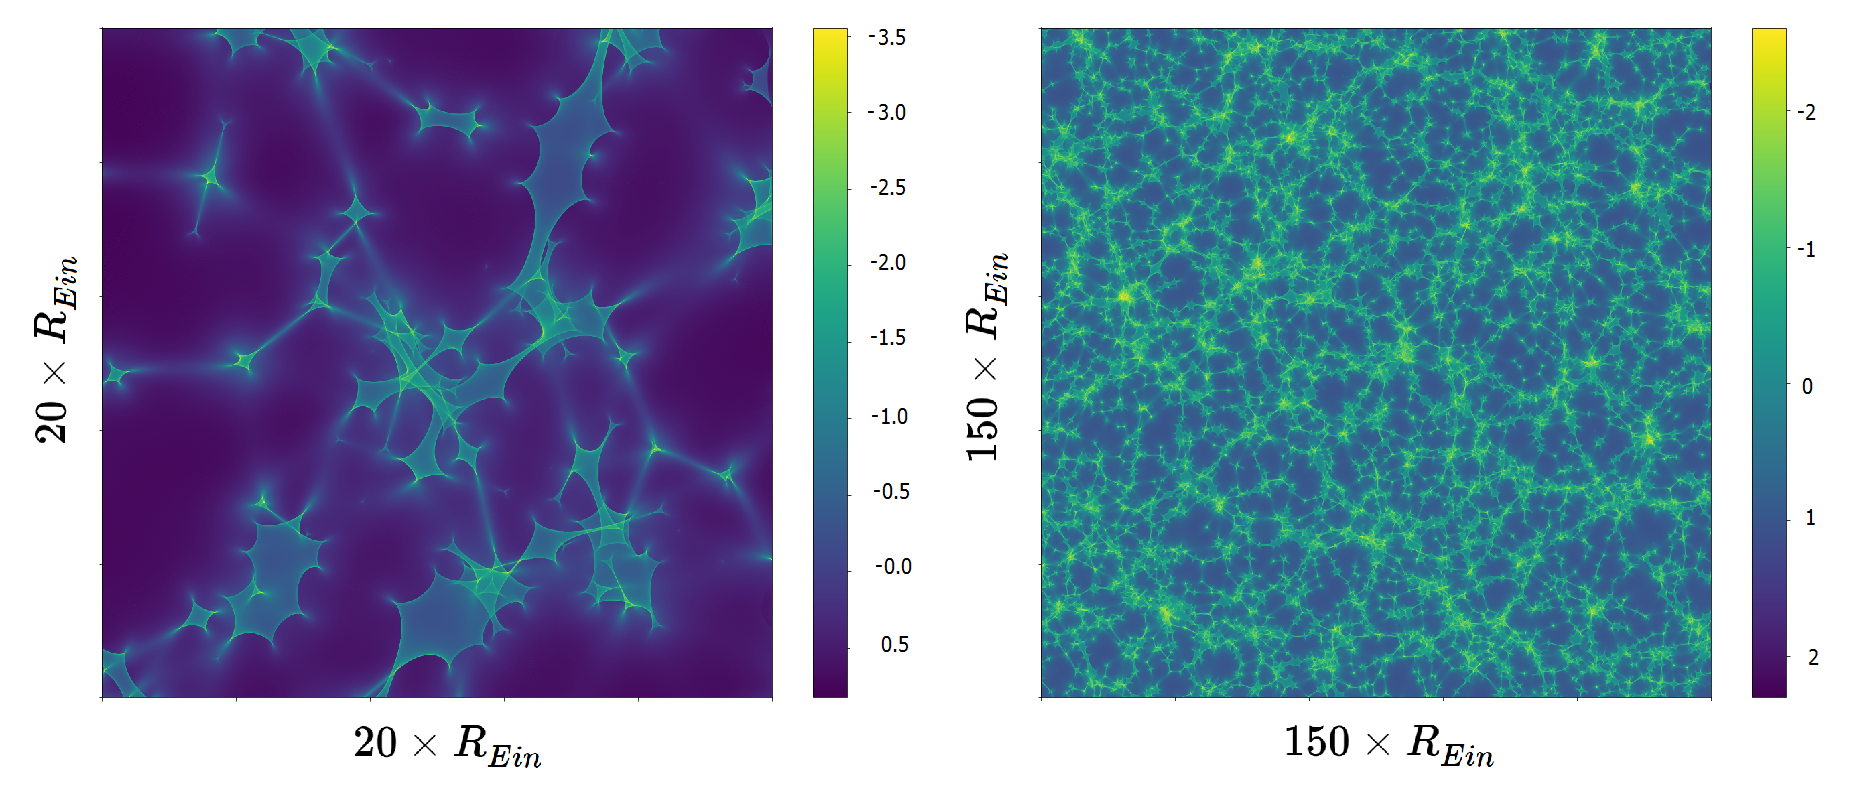
\includegraphics[scale=0.22]{pics/maps_example.png}
%	\caption{Карты микрокаустик. Количество звёзд-линз слева - 313, справа - 14526. Цветовая шкала (в единицах звёздных величин) показывает, как дополнительно увеличивается или ослабляется яркость источника вследствие только микролинзирования. \label{fig:micromaps}} 
%\end{figure}

